\subsection{Heuristik}
Wir entwickeln ein heuristisches Verfahren, um diesem Problem zu begegnen. 
Wir lassen zuerst einen Greedy--Algorithmus laufen, um ein Ausgangsergebnis zu erzeugen und
danach führen wir einen Bergsteigeralgorithmus (engl. \textit{hill climbing algorithm}) aus,
der das Ausgangsergebnis heuristisch optimiert, indem er ein lokales Maximum durch mehrmalige
Mutationen findet.
\TODO{Vielleicht doch ein besserer Algorithmus? Testen!} 


\subsubsection{Greedy--Algorithmus}
Wie schon im \cref{sec:definitionen} erwähnt wurde, können die Gedanken bezüglich des
\fp{} auf andere Größen übetragen werden. Da die Größen des Rechtecks $R$ sowie des Zeitraums fest sind
und auf 1000 Metern bzw. auf den Zeitraum von 8:00 is 18:00 beschränkt sind, konvertieren wir
die Eingabe, indem wir den Beginn des Zeitraumes auf 0 setzen, d.h., wir subtrahieren den 
Anfang $B$ vom Ende $E$. So bleibt auch der WErt $M$, also die Differenz von $E$ und $B$, gleich. 
Analog müssen wir Eingabe der kleineren Rechtecke $r_i$ entsprechend konvertieren, indem wir
von jedem $b_i$ und $e_i$ den Wert $B$ abziehen. Für"die Aufgabe hat diese Konversion keine
Bedeutung und funktioniert auch, wenn ein angegebener Zeitraum sich vom ursprünglichen Zeitraum unterscheidet.
Mit dieser Konversion können wir ebenfalls mehrtägige Flohmärkte oder
sogar mehrere unterschiedlichen Flohmärkte behandeln.
Wenn der angegebene Zeitraum an einer Stelle unterbrochen ist,
etwa von 7:00 bis 9:00 und dann von 12:00 bis 15:00, ist es auch kein Problem, dann kann der
Zeitraum von 7:00 bis 15:00 angegeben werden und die Zeiten zwischen 9:00 und 12:00 bleiben unbesetzt.
Mehrtägige Flohmärkte können auf dieselbe Weise behandelt werden: Die gesamte Öffnungszeiten des Flohmarktes können in Stunden angegeben werden, zum Beispiel der Zeitraum eines Flohmarkts, der zwei Tage von 10:00 bis 17:00 dauert, kann als von 10:00 bis 41:00 (17:00 + 24 Stunden) dargestellt werden. Mehrere unterschiedlichen Flohmärkte kann man analog kodieren. Es hängt nur von der Eingabe ab.
\TODO{Beipiele dazu}
\TODO{Erwähne Zeiten in Minuten}
Nach der Konversion der Eingabe bilden wir eine Liste $Z$, in der jedes
Rechteck $r_i$ mit seinen genannten Größen $s_i, b_i, e_i$ gespeichert.

Die Größen $N$ und $M$ sind im Programm fest, unabhängig davon, wie viel sie betragen.
Außerdem wurde im \cref{sec:definitionen} festegestellt, dass die Größen $s_i$, $b_i$ und $e_i$
des jeweiligen Rechtecks $r_i$ fest sind und dass wir nur ein Rechteck $r_i$ entlang der $x$--Achse,
also entlang der Seite der Länge $N$ des Rechtecks $R$ bewegen dürfen.
So bietet sich eine Verteilung der kleinere Rechtecke $r_i$ auf kleinere \textit{\textbf{Streifen}}
der Länge $N$ im Rechteck $R$ entlang der Seite der Länge $N$.
Die Breite eines solchen Streifen ist äquidistant für alle Streifen und, da
man Stände am Flohmarkt nur zu vollständigen Stunden vermieten kann, lässt sich
die Breite eines Streifens zu einer vollständiger Stunde bstimmen.
\TODO{Minuten erwähnen}
Im Programm sind diese Streifen einfach Listen mit allen kleineren Rechtecken, 
deren Breite $m_i$ sich in diesem Streifen enthält.
Legen wir die folgende Schreibweise fest: Ein Streifen im Rechteck $R$, der die
Stunde $k$ betrifft, also in der Stunde $k$ beginnt und in der Stunde $k+1$ endet, nennen wir $S_k$.
Das bedeutet, dass ein Rechteck von $b_i = 1$ (nach Konversion, in vollständigen Stunden)
und $e_i = 5$ in den folgenden Streifen enthalten wird: $S_1, S_2, S_3, S_4$. Im Streifen $S_5$
wird er nicht enthalten, da die Miete mit dem Anfang der 5. Stunde endet.
Wie Streifen implementiert werden, lesen Sie in der \nameref{sec:umsetzung}.

Nach dieser Vorbereitung der Eingabe erfolgt der Lauf unseres Greedy--Algorithmus, der das
Ausgangsergebnis liefert.
Wir sortieren die Rechtecke in jeder Liste $S_i$ unabhängig voneinander nach folgenden Kriterien
in dieser Reihenfolge: 
1) fallend nach dem Wert $e_i$,
2) aufsteigend nach dem Wert $b_i$ und
3) fallend nach der Fläche jedes Rechtecks. 
Somit sind die ersten Rechtecke in jeder Liste $S_i$ diejenigen,
deren Wert $e_i$ am größten ist --- oft diejenigen, die am breitesten im Streifen sind.
\TODO{warum diese Reihenfolge? najpierw załatwaimy od lewej największe, po prawej upychamy najmniejszymi}
Diese Reihenfolge wurde so gewählt, dass wir in dieser Reihefolge versuchen,
die Rechtecke aus den Streifen ins große Rechteck $R$ zu platzieren.

Stellen wir uns vor, die das Rechteck $R$ liegt auf auf einem Koordinatensystem.
Die Seite der Länge $N$ verläuft entlang der $x$--Achse und die Seite der Länge
$M$ entlang der $y$--Achse.
Der Wert $B$ (nach der Konversion) wird entsprechend am Punkt $(0, 0)$ abgebildet.
Wir verarbeiten Streifen für Streifen in der
aufsteigenden Reihenfolge der $y$--Werte beginned mit dem 0--ten Streifen.
Wir iterieren durch jede Liste $S_i$ und untersuchen jedes Rechteck $r_j$ in diesem
Streifen, ob sein Wert $b_j$ gleich dem Wert $i$, also ob das Rechteck (die Anmeldung) mit dem
aktuellen Zeitpunkt $i$ beginnt. Außerdem prüfen wir, ob ein Rechteck bereits platziert wurde.
Wenn ein 



Damit kann man sich vorstellen, dass wir das Rechteck $R$ quasi vom Punkt $(0,0)$ bis zum Punkt
$(N, E)$ mit kleineren Rechtecken füllen. Nach 

\begin{figure}[h]
\centering
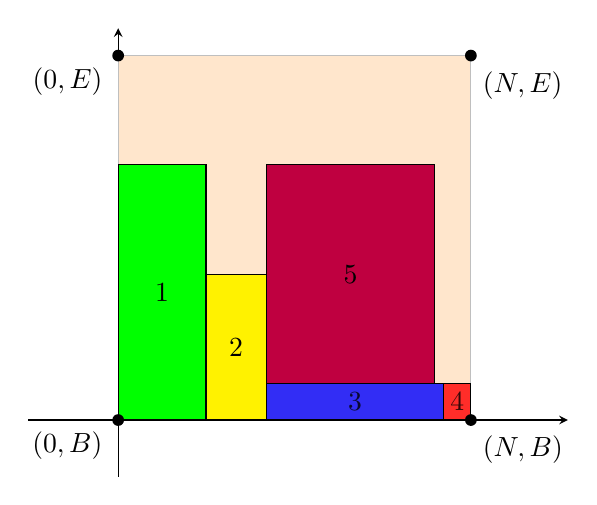
\begin{tikzpicture} 
\begin{axis}[
		ticks=none,
        xmin =-2.55,
        xmax = 12.75,
        ymax = 10.75,
        ymin = -1.55,
        axis x line = middle, axis y line = middle,
        every axis plot/.append style={ultra thick}]

	\draw [draw=lightgray, fill=orange, fill opacity=0.2] (0,0) rectangle (10, 10);
	\draw [fill = green] (0,0) rectangle node {1} (2.49, 7) ;
	\draw [fill = yellow] (2.49, 0) rectangle node {2} (4.2, 4) ;
	\draw [fill = blue, fill opacity = 0.8] (4.2, 0) rectangle node {3} (9.23, 1) ;
	\draw [fill = red, fill opacity = 0.8] (9.23, 0) rectangle node {4} (10, 1) ;
	\draw [fill = purple] (4.2, 1) rectangle node {5} (8.97, 7) ;
	\node[label={200:{$(0, B)$}},circle,fill,inner sep=1.5pt] at (axis cs:0,0) {};
	\node[label={290:{$(N, B)$}},circle,fill,inner sep=1.5pt] at (axis cs:10,0) {};
	\node[label={200:{$(0, E)$}},circle,fill,inner sep=1.5pt] at (axis cs:0,10) {};
	\node[label={290:{$(N, E)$}},circle,fill,inner sep=1.5pt] at (axis cs:10,10) {};
	%\draw [fill = yellow] (0,7) rectangle node {} (5.26, 10) ;
\end{axis} 
\end{tikzpicture}
\end{figure}




\TODO{wie werden die Rechtecke gelegt?\\
-- binary search\\
-- was sind die Folgen? was will man damit erreichen?}




\subsubsection{Heuristisches Verbesserungsverfahren}\label{sec:verbesserung}
Man kann leicht feststellen, dass, wenn alle Rechtecke aus $Z$ im Laufe des
Greedy--Algorithmus in $R$ platziert wurden oder wenn die ganze Fläche von $R$ bedeckt wurde, 
das Problem für diese Eingabe optimal gelöst wurde.
Allerdings lässt sich nicht nachweisen, dass der vorgestellte Algorithmus 
stets eine optimale Platzierung liefert.
Hingegen kann man sogar festellen, dass es bessere Ergebnisse gibt als die,
die am Anfang geliefert werden. 


Wir probieren, das Ausgangsergebnis heuristisch zu verbessern.
Bezeichnen wir ab jetzt ein beliebiges Ergebnis, also eine beliebige Anordnung
der kleineren Rechtecke innerhalb des großen Rechtecks $R$, die unser Programm liefert, 
als $C$. Insbesondere nennen wir unser Ausgangsergebnis $C_A$.


Offensischtlich kann man mithilfe des obengenannten Greedy--Algorithmus 
das Ausgangsergebnis nicht optimieren. Wir haben begründet, dass dieser Algorithmus
an jeder Stelle stets die aktuell optimale Variante wählt. 
Außerdem dürfen wir diesen Algorithmus nicht nochmals nutzen,
da wir voraussetzen, dass die Streifen in der aufsteigender Reihenfolge einer nach dem anderen
verarbeitet werden. Dann kann es sein, dass sich eine Lücke der Länge $\ell$
zwischen zwei Punkten $(x_j, j)$ und 
$(x_j + \ell, j)$ in einem Streifen $j$ befindet
und dass ein Rechteck $r_i$ mit $s_i \leqslant \ell$ theoretisch hineinpassen würde, aber
es ist nicht mehr gesichert, dass es die Lücken direkt darüber in oberen Streifen $j+1, j+2, ...$
geben würde.


Deshalb führen wir ein neues Verfahren ein. 
Sei $C$ eine beliebige Platzierung von Rechtecken innerhalb von $R$.
Nennen wir $C$ \textit{das aktuelle Ergebnis}. 
Die allgemeine Idee lautet:
Ein nicht platziertes Rechteck $r$ wird in $R$ platziert, ggf. 
alle Rechtecke, die mit $r$ kollidieren, werden aus $R$ entfernt und
die neu entstandenen Lücken werden mit nicht gelegten Rechtecken gefüllt. 
So kommt man auf einen neuen Zustand $C'$, also eine neue Platzierung der Rechtecke.
Es wird dann überprüft, ob der Gesamtflächeninhalt aller platzierten Rechtecke in der Platzierung $C'$
größer ist als der in der Platzierung $C$.
Wenn ja, wird $C'$ das aktuelle Ergebnis und der Vorgang wiederholt sich,
bis es nicht mehr möglich ist, einen Zustand $C$ weiter zu verändern.
Wir sehen, dieser Ansatz nimmt viel Inspiration aus der Idee der Bersteigeralgorithmen,
dennoch lässt er sich schlecht als einer klassifizieren.
Unser Algorithmus ist zu deterministisch,
es fehlen starke Mutationen in seinen Lauf, die das Ergebnis deutlich beinflussen könnten,
und es fehlen Anwendungen der Randomisierung.


Wie kommt es zur Veränderung der Platzierung und wann bestimmen wir,
dass es unmöglich ist, einen Zustand weiter zu verändern?
Unser Verbesserungsverfahren arbeitet mit Lücken, die 
nach der Platzierung $C_A$ entstehen.
Die Idee ist, man findet eine Lücke in einem Streifen 
und man legt ein noch nicht platziertes Rechteck $r$ in die Lücke,
ggf. muss man die Rechtecke,
die mit $r$ kollidieren, aus der Platzierung entfernen
und somit entstehen neue Lücken,
die mit anderen nicht gelegten Rechtecken gefüllt werden können.
So kommt man auf ein neues Ergebnis.
Man hört auf, wenn es keine Lücken mehr gibt, für die ein Rechteck zum Platzieren zur Verfügung steht.


Zuerst muss man die nicht platzierten Rechtecke für jeden Streifen bestimmen. 
So legen wir für jeden Streifen $j$ eine Liste $U_j$ fest, in der sich alle 
Rechtecke aus dem Streifen $j$ befinden, die nicht platziert sind.
Die Liste $U_j$ muss man auf eine bestimmte Weise ordnen.
Jedes Rechteck $r_i$ in jeder solchen Liste sortieren wir nach diesen Kriterien:
1) aufsteigend nach der Länge $s_i$ und 2) aufsteigend nach dem Beginn $b_i$.
Die Entscheidung, diese Sortierkriterien zu wählen, ergibt sich experimentell 
und wird im \cref{sec:diskussion-ergebnisse} diskutiert.


Danach muss man die Lücken in jedem Streifen in einer Platzierung finden.
So legen wir eine Liste $H_j$ für jeden Streifen $j$ fest, in der sich alle
Lücken aus diesem Streifen befinden. Man findet sie, indem
man durch jedes im Streifen $j$ platziertes Rechteck $r_i$ iteriert und jeweils überprüft,
ob das Rechteck $r_i$ mit dem Rechteck $r_{i+1}$ eine gemeinsame Seite haben. Wenn nicht, gibt es eine Lücke
zwischen den Rechtecken $r_i$ und $r_{i+1}$.
Dazu muss man auch untersuchen, ob das erste Rechtecks 
und das letzte Rechteck im Streifen direkt an den Seiten des großen Rechtecks liegen. 
Wenn nicht, enstehen auch Lücken zwischen den Rechtecken und den Seiten des großen Rechtecks $R$.  

Danach werden alle Listen $H_j$ zu einer Liste $H$ zusammengebracht.
Diese Liste muss auch auf eine bestimmte Weise geordnet sein. 
Experimentell ergeben sich die folgenden Sortierkriterien für jede Lücke $L_i$: 
1) fallend nach der Größe der Lücke $L_i$ und 2) aufsteigend nach dem
Index des Streifens. Diese Entscheidung wird ebenfalls im \cref{sec:diskussion-ergebnisse}
diskutiert.

\begin{algorithm}[h]
\caption{Das heuristische Verbesserungsvefahren}
\label{algo:verbesserung}
\flushleft
\textbf{Eingabe:} $R$ --- das große Rechteck, $Z$ --- die Liste mit allen kleineren Rechtecken.
\begin{algorithmic}[1]
\State $C_A \gets$ Greedy($R, Z$)
\State $H \gets$ getAllHoles$(C_A)$
\State $U \gets$ getRecs$(C_A)$
\State $C \gets C_A$
\State $itH \gets H.begin$
\State $j \gets itH.$Streifen\Comment{$j$ ist der Index des Streifens, in dem sich die Lücke zum Iterator $itH$ befindet}
\State $itR \gets U_j.begin$
\While{$itH \neq H.end$}\label{line:abbruch}
	\State $\Sigma_C \gets |C|$ \Comment{der Gesamtflächeninhalt aller platzierten Rechtecke in $C$}
	\State $C' \gets$ next$(C, itH, itR)$
	\State $itR \gets itR + 1$
	\State $\Sigma_{C'} \gets |C'|$
	\If {$\Sigma_{C'} > \Sigma_C$} \label{line:vergleich}
		\State $H \gets$ getAllHoles$(C')$
		\State $U \gets$ getRecs$(C')$
		\State $itH \gets H.begin$
		\State $k \gets itH.$Streifen
		\State $itR \gets U_j.begin$
		\State $C \gets C'$
	\EndIf
\EndWhile
\end{algorithmic}
\end{algorithm}

Der \cref{algo:verbesserung} zeigt eine vereinfachte Vorgehensweise des Verbesserungsverfahrens.
Die Funktion $getAllHoles(C)$ findet alle Lücken in allen Streifen im Rechteck $R$ in der
aktuellen Platzierung $C$ und bestimmt die Liste $H$.
Die Funktion $getRecs(C)$ findet alle nicht platzierten Rechtecke und verteilt sie auf
die Listen $U_j$ für jeden Streifen $j$.
Die Funktion $next(C, itH, itR)$ besteht in diesem Algorithmus selbst aus drei Funktionen,
die im Folgenden beschrieben werden.

Die erste Funktion bestimmt die nächste Lücke, in die ein nicht platziertes Rechteck 
eingefügt wird. Es gibt einen Iterator $itH$, der am Anfang am Beginn der Liste $H$ gesetzt wird.
Im Laufe des Algorithmus bewegt sich der Iterator und zeigt auf nächste Lücken.
Eine Lücke bezeichnen wir als \textit{geeignet}, wenn sie sich in einem
Streifen $j$ befindet, zu dem die entsprechende Liste $U_j$ nicht leer ist, d.h., 
es gibt mindestens ein Rechteck, das in diese Lücke eingefügt werden kann.
Somit bewegt sich der Iterator in der Liste $H$ und wenn er auf eine geeignete Lücke 
stößt, wird diese Lücke durch die folgenden zwei Funktionen bearbeitet.
Insbesondere beachte man, dass die While--Schleife in \cref{line:abbruch} abbricht, wenn
der Iterator $itH$ zum Ende der Liste $H$ gelangt, also dann,
wenn es keine geeigneten Lücken mehr gibt. 

Die nächste Funktion wählt ein Rechteck $r$, das in eine gewählte geeignete Lücke $L$
eingefügt wird. Da die gewählte Lücke sich in einem Streifen $j$ befindet, stammt $r$
aus der Liste $U_j$.
Es gibt auch einen internen Iterator $itR$ für die Liste $U_j$,
der bei jeder neuen Lücke an den Anfang der Liste gesetzt wird.
Wenn ein Rechteck $r$ in einem Lauf $t$ der While--Schleife in $L$ eingefügt wird,
wird $itR$ danach inkrementiert und im darauf folgenden Lauf der 
Schleife $t+1$ wird ein unterschiedliches Rechteck in die Lücke $L$ gelegt.
Wenn der Iterator $itR$ bis zum Ende der Liste $U_j$ gelangt, wird der Iterator $itH$
in der Liste $H$ inkrementiert und somit eine neue 
geeignete Lücke gesucht.

Die letzte Funktion nimmt das unter dem Iterator $itR$ stehende Rechteck $r$
und legt es in die unter dem Iterator $itH$ stehende Lücke $L$.
Diese Funktion bereitet eine neue Platzierung $C'$ vor.
Seien die Koordinaten der Lücke $x_1$ und $x_2$ und der Streifen, in dem sich $L$ befindet, sei $j$. 
Seien $x_r$ und $x_r + s_r$ die $x$--Koordinaten von $r$.
Das Rechteck $r$ wird in $R$ so gelegt, dass $x_2 = x_r + s_r$. Auf diese Weise beträgt
der Wert $x_r \coloneqq x_2 - s_r$.\footnote{Die Situation, in der $x_r < 0$ gilt, wird  in der
zweiten Funktion ausgeschlossen. Wenn es dazu käme, wird der Iterator $itR$ inkrementiert wird und das nächste Rechteck gewählt.}
Selbstverständlich kann es an dieser Stelle zu Kollisionen kommen --- Rechtecke können sich überdecken.
Vor dem Platzieren prüft man nicht, ob es durchgehend eine Lücke zwischen den Werten $x_r$ und $x_r + s_r$ 
in allen Streifen $k$ gibt, wobei $b_r \leqslant k < e_r$.
Deshalb entfernt man nun alle Rechtecke, die mit $r$ kollidieren, also all diejnigen, die 
zumindest zum Teil zwischen $x_r$ und $x_r + s_r$ in einem Streifen $k$ liegen.
So entstehen auch neue Lücken, deshalb versuchen wir an dieser Stelle 
die Lücken mit anderen Recktecken zu füllen.
Dazu verarbeiten wir alle Streifen $k$ ($b_r \leqslant k < e_r$), indem wir
jedes in $C'$ noch nicht gelegte Rechteck $r_i$
in jeder Liste $S_k$ (in der ursrpünglichen Reihenfolge) untersuchen.
Wie beim Greedy--Algorithmus am Anfang versuchen wir, ein Rechteck
$r_i$ im Streifen $g$ zu legen nur, wenn $g = b_i$
(und wenn es eine Lücke zwischen $x_{r_i}$ und $x_{r_i} + s_i$ gibt).
Allerdings müssen wir die Streifen $b_i+1, b_i+2, ..., e_i-1$ vor dem Platzieren prüfen,
ob es in ihnen durchgehend Lücken zwischen $x_{r_i}$ und $x_{r_i} + s_i$ gibt. 
Nur, wenn in allen Streifen $b_i, b_i + 1, ..., e_i-1$ diese Lücken bestehen,
kann das Rechteck $r_i$ in die Platzierung $C'$ eingefügt werden. 
Nachdem alle durch Kollision betroffenen Streifen verarbeitet worden sind,
ist die Platzierung $C'$ fertig.

Dann erfolgt der Vergleich in \cref{line:vergleich}.
Wenn der Gesamtflächeninhalt der Platzierung $C'$ streng größer ist als
der Gesamtflächeninhalt der Platzierung $C$, wird die neue Platzierung vom Algorithmus
akzeptiert und gilt als die aktuelle Platzierung $C$.
Danach muss man offensichtlich alle Lücken und alle nicht gelegten Rechtecke neu bestimmen.
Die Iteratoren $itH$ bzw. $itR$ werden auf $H.begin$ bzw. auf $U_k.begin$ gesetzt. 

Man kann leicht begründen, dass das Programm auf jeden Fall anhält.
Durch den Quasibergsteigeralgorithmus wird ein lokales Maximum gefunden, das bestenfalls auch
das Optimum ist. 
Jedes lokale Maximum kann das Optimum nicht überschreiten.
Das Optimum ist auf den Flächeninhalt des großen Rechtecks $R$ beschränkt.
Wenn ein lokales Maximum erreicht wird, kann der Algorithmus keine neuen Platzierungen
annehmen. 
Wenn ein lokales Maximum erreicht wird, werden alle geeigenten Lücken und dazu jeweils alle 
passenden Rechtecke ausprobiert, aber das Programm nimmt keine der neuen Kombinationen an,
da sie keinen größeren Flächeninhalt bilden als der des lokalen Maximums.
Somit hält das Programm auf jeden Fall an.
 












